\lstset{language=Alloy}.



\section{Alloy Model}
In this section we show the model of the system, by formalizing it with Alloy. This step is strictly important, due to the consistency of our model. 
In particular it describes the basic structure and the behavior of our system based on FOL.
Our model aims to describe the users's dynamics inside and outside the market in an arbitrary day with their attributes about their bookings.
The main model's aspect described are the following:

\begin{itemize}
\item Users enters in the market with a QRCode if and only if it's valid but not submitted yet. Otherwise, with different boolean values the QRCode signature could have different meaning. All possibile type of QRCode could be:
    \begin{itemize}
    \item \textit{valid and not submitted}: QRCode owner has booked an appointment (either a Reservation or a Visit) and he hasn't entered yet;
    \item \textit{submitted and valid}: the QRCode owner is in the market ;
    \item \textit{submitted and not valid}: the QRCode is already used by the owner;
    \end{itemize}
\item The model is organized temporaly in time slots of 30 minutes each. This way make easier the Visit schedule;
\item The time estimation of each appointment is determined by the bag size. In particular it could be:
\begin{itemize}
\item \textit{Small}: it occupies 1 slot in the schedule, that is 30 minutes;
\item \textit{Medium}: it occupies 2 slots in the schedule, that is 60 minutes;
\item \textit{Large}: it occupies 3 slots in the schedule, that is 90 minutes;
\end{itemize}

\item Users in the queue are put in order depending on his booking number. Smaller is  the booking number higher will be the priority with which the user will enter in the market;

\item Given the timetable of the Visit, only 3 users are allowed to enter in the market with a Visit in the same time. However, this will not formalized in our model due to the fact that it needs a too large number of users in the simulation, which is technically hard for the Alloy tool;

\end{itemize}

\lstinputlisting[language=alloy]{model/alloy.als}




\section{Alloy Results}



\begin{figure}[H]
  \label{marketOpened}
  \centering
  \makebox[\linewidth]{
  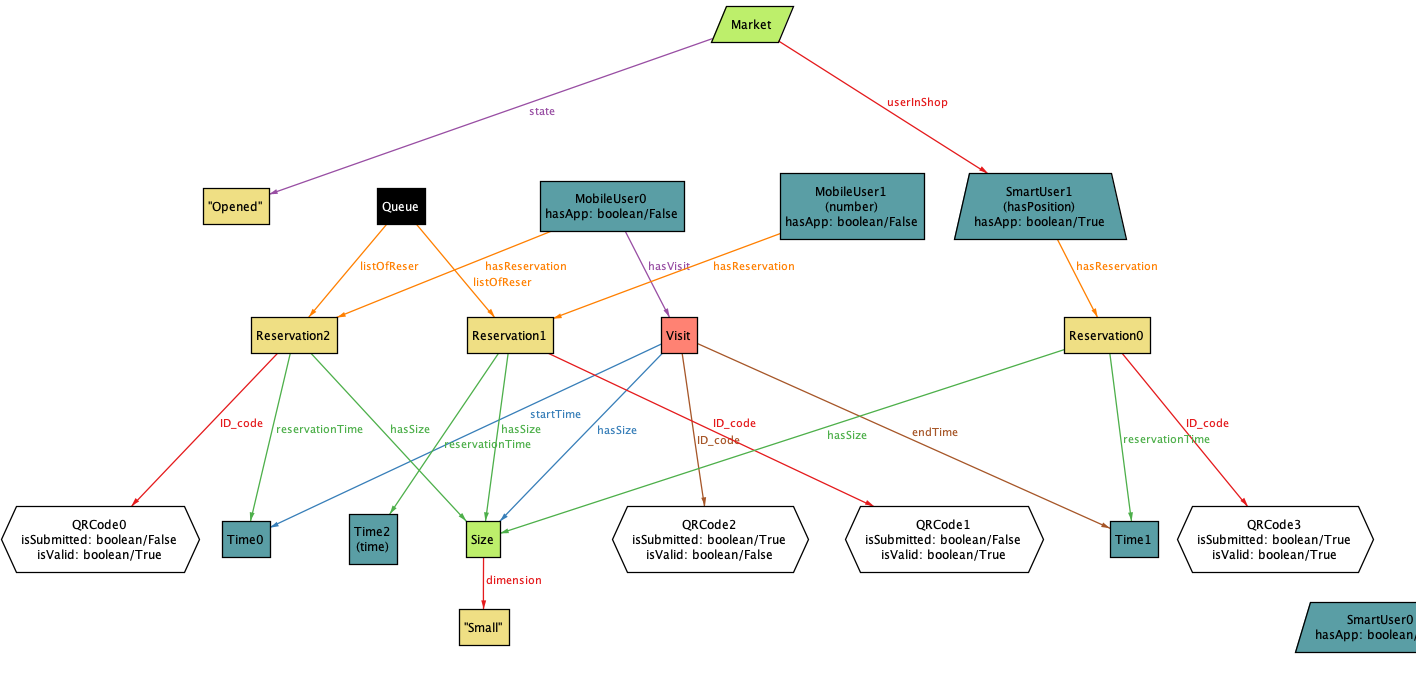
\includegraphics[scale=0.52]{report_alloy/marketOpened.png}}
    \caption{...}
\end{figure}

\begin{figure}[H]
  \label{marketClosed}
  \centering
  \makebox[\linewidth]{
  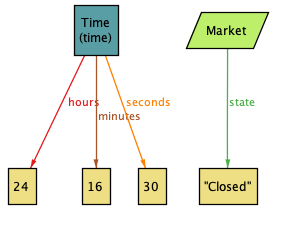
\includegraphics[scale=0.52]{report_alloy/marketClosed.png}}
    \caption{...}
\end{figure}

\begin{figure}[H]
  \label{shorReserv}
  \centering
  \makebox[\linewidth]{
  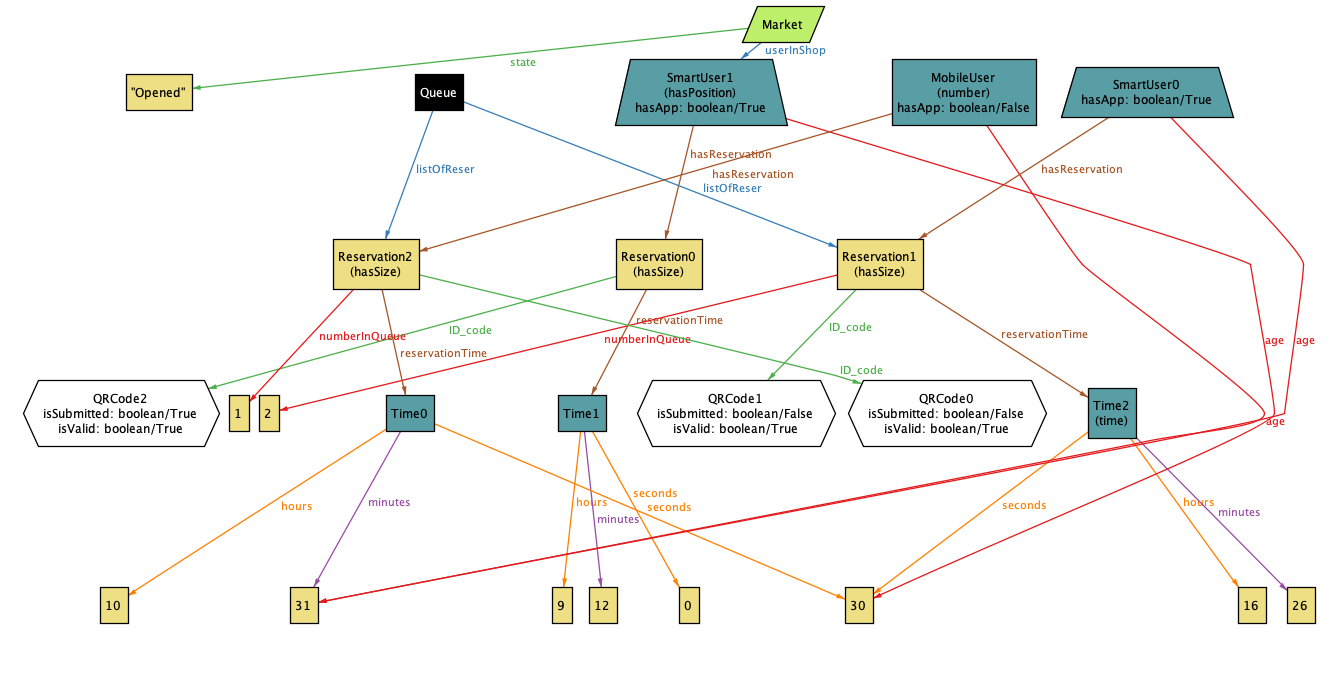
\includegraphics[scale=0.52]{report_alloy/shorReserv.png}}
    \caption{...}
\end{figure}

\begin{figure}[H]
  \label{showVisit}
  \centering
  \makebox[\linewidth]{
  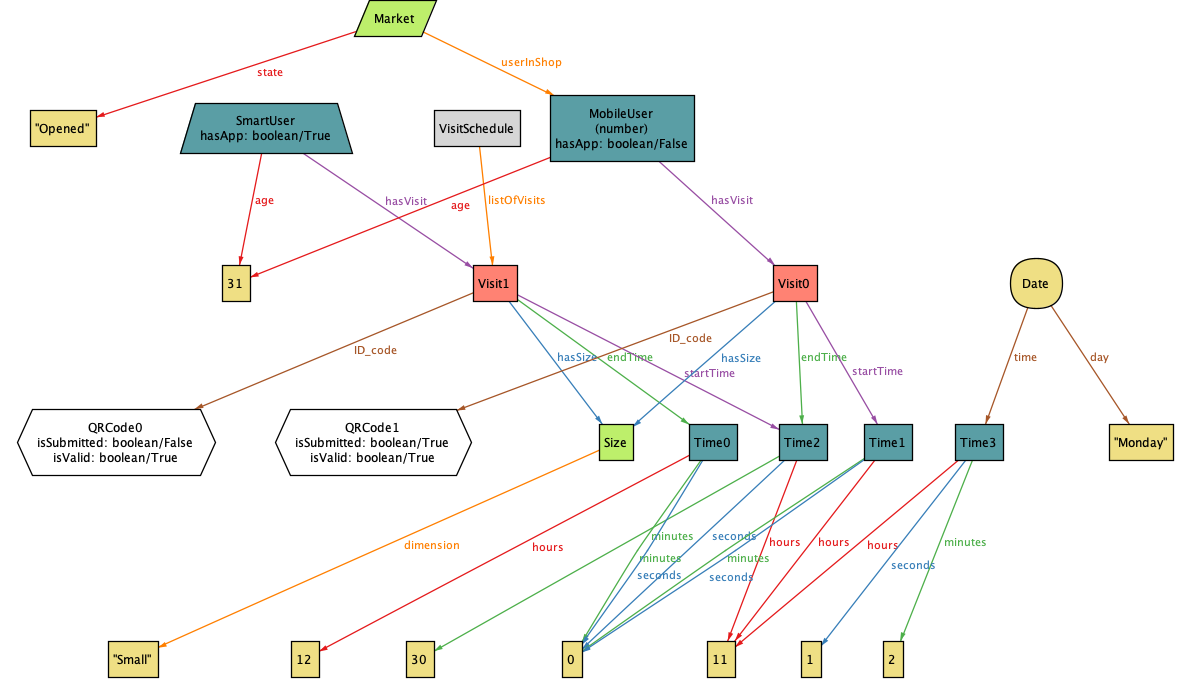
\includegraphics[scale=0.52]{report_alloy/showVisit.png}}
    \caption{...}
\end{figure}


\begin{figure}[H]
  \label{addInQueue}
  \centering
  \makebox[\linewidth]{
  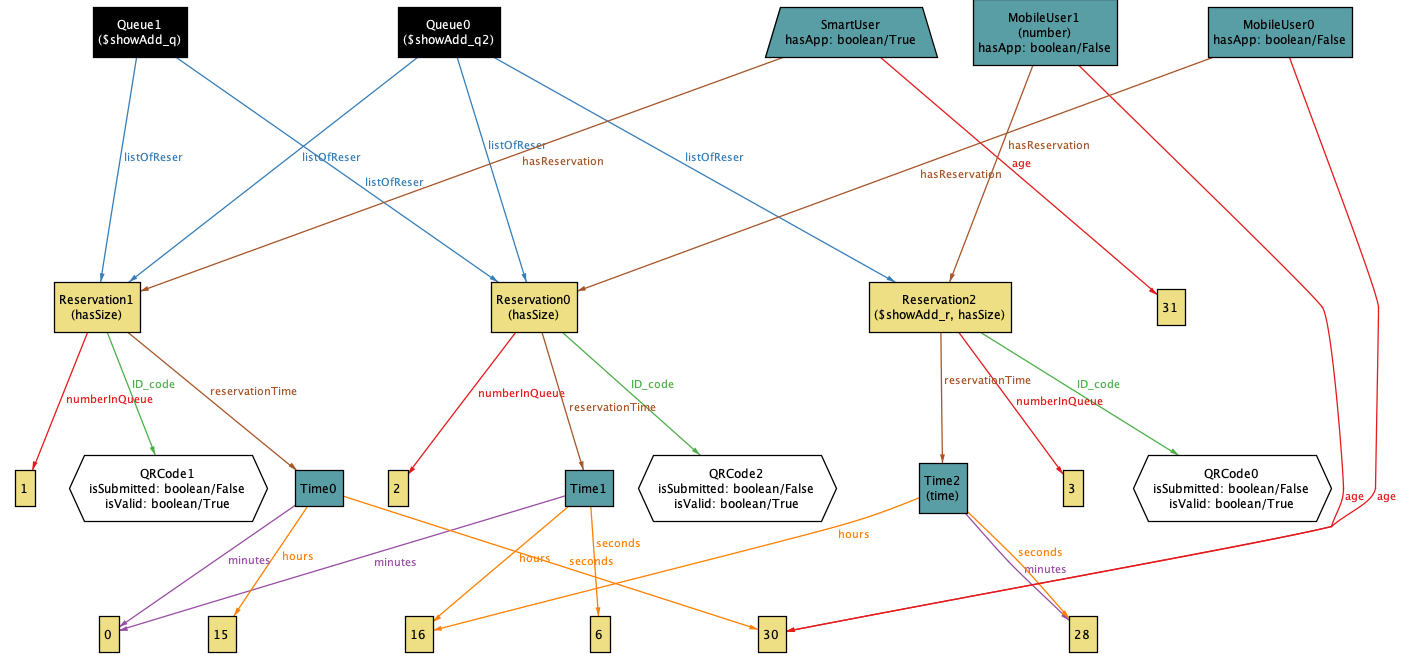
\includegraphics[scale=0.52]{report_alloy/addInQueue.png}}
    \caption{...}
\end{figure}


\begin{figure}[H]
  \label{deInQueue}
  \centering
  \makebox[\linewidth]{
  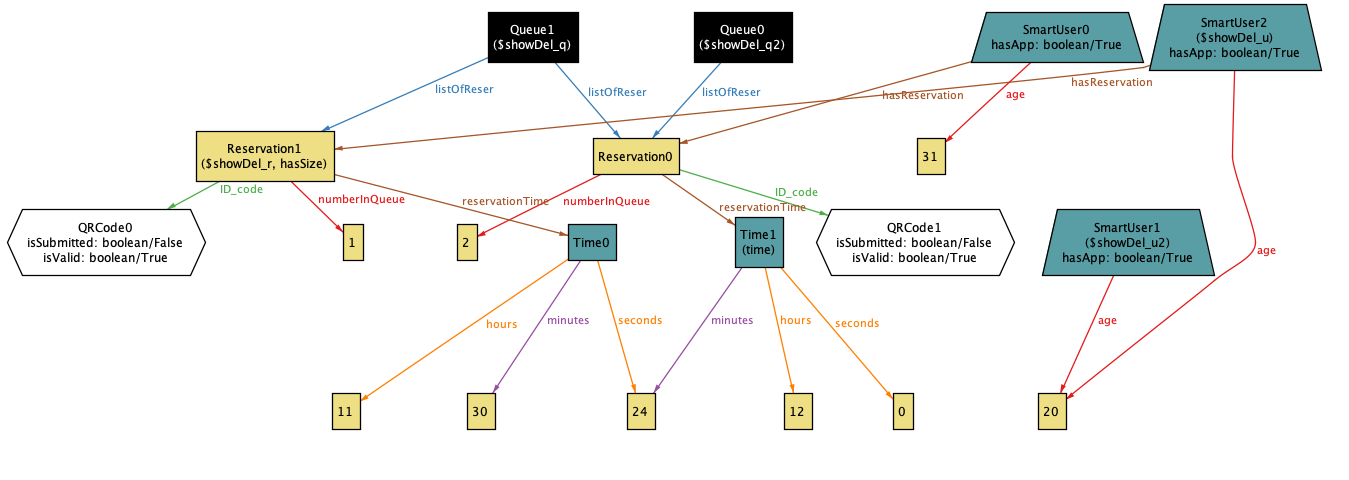
\includegraphics[scale=0.52]{report_alloy/deInQueue.png}}
    \caption{...}
\end{figure}


\begin{figure}[H]
  \label{pred1}
  \centering
  \makebox[\linewidth]{
  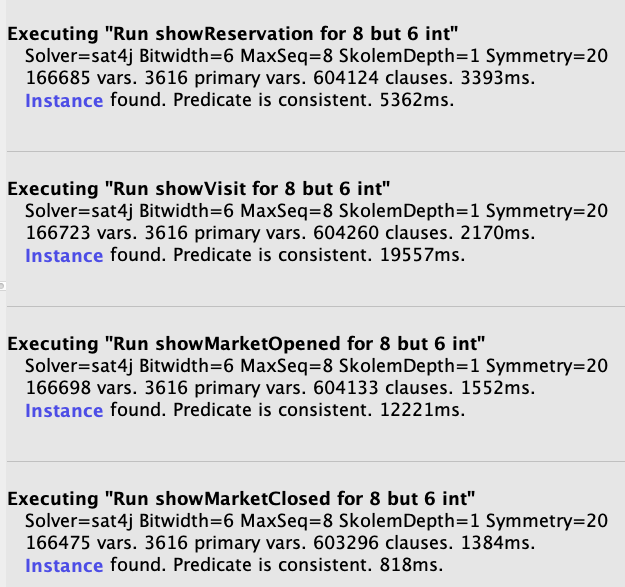
\includegraphics[scale=0.52]{report_alloy/pred1.png}}
    \caption{...}
\end{figure}

\begin{figure}[H]
  \label{pred2}
  \centering
  \makebox[\linewidth]{
  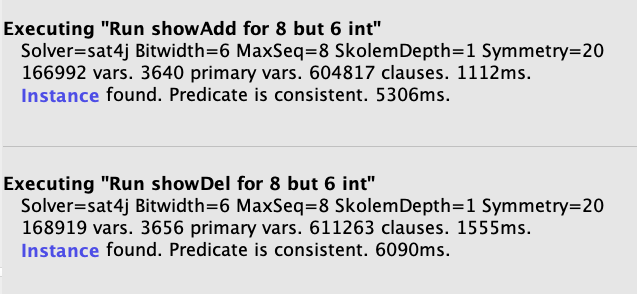
\includegraphics[scale=0.52]{report_alloy/pred2.png}}
    \caption{...}
\end{figure}

\begin{figure}[H]
  \label{reportAssert}
  \centering
  \makebox[\linewidth]{
  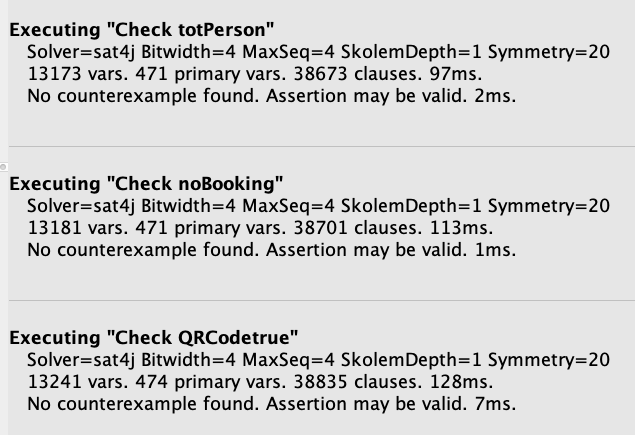
\includegraphics[scale=0.52]{report_alloy/reportAssert.png}}
    \caption{...}
\end{figure}